
\chapter{Statistics and Probability}
\subsection{Definition of Moments}
Let $x\in\mathbb R^{n}$ is a random variable.
We write $m = E[x]\in\mathbb R^n$ for the expectation and
$M=\mathrm{Var}[x] = E[(x-m)(x-m)^T]$ for the covariance (when these quantities are defined.)

In tensor diagrams, we will use square brackets:
\[
\mathbin{\begin{tikzpicture}[baseline=(n0.base), inner sep=1pt]
   \node (n0) at (0,0) {$m=[$};
   \node [right=1em of n0] (n1) {$x]$};
   \draw (n0) -- (n1);
\end{tikzpicture}}
\quad\text{and}\quad
\mathbin{\begin{tikzpicture}[baseline=(n0.base), inner sep=1pt]
   \node (n0) at (0,0) {$M=[$};
   \node [right=1em of n0] (n1) {$(x\ominus m)$};
   \node [right=.5em of n1] (n2) {$(x\div m)$};
   \node [right=1em of n2] (n3) {$]$};
   \draw (n0) -- (n1);
   \draw (n2) -- (n3);
\end{tikzpicture}}
\]
Note we used the German minus, $\div$, to distinguish subtraction from contraction edges.

We can also define the third and fourth centralized moment tensors
\[
   M_3=
   \renewcommand*{\arraystretch}{1.3}
   \begin{bmatrix}
      \vecmatvec{1em}{(x\div m)}{}{} \\
      \vecmatvec{1em}{(x\div m)}{}{} \\
      \vecmatvec{1em}{(x\div m)}{}{}
   \end{bmatrix}
\quad\text{and}\quad
M_4=
   \renewcommand*{\arraystretch}{1.3}
   \begin{bmatrix}
      \vecmatvec{1em}{(x\div m)}{}{} \\
      \vecmatvec{1em}{(x\div m)}{}{} \\
      \vecmatvec{1em}{(x\div m)}{}{} \\
      \vecmatvec{1em}{(x\div m)}{}{}
   \end{bmatrix}
.
\]

\subsection{Expectation of Linear Combinations}
General principle: The ``linearity of expectation'' lets you pull out all parts of the graph not involving $X$.

\subsubsection{Linear Forms}
\begin{align*}
   \tag{312}
   \E[AXB+C] &= A \E[X] B + C
   &
   \renewcommand*{\arraystretch}{1.3}
   \begin{bmatrix}
      \matmul{A,X,B} \\+\, \matmul{C}
   \end{bmatrix}
   &=
   \renewcommand*{\arraystretch}{1.3}
   \begin{matrix}
      \matmul{A,[X],B} \\+\, \matmul{C}
   \end{matrix}
   %%%%%%%%%%%%%%%%%%%%%%%%%%%%%%%%%%%%%%%%
   \\
   \tag{313}
   \mathrm{Var}[Ax] &= A \mathrm{Var}[x] A^T
   &
   \renewcommand*{\arraystretch}{1.3}
   \begin{bmatrix}
      \vecmatvec{.5em}{A}{}{x} \div [\vecmatvec{.5em}{A}{}{x}] \\
      \vecmatvec{.5em}{A}{}{x} \div [\vecmatvec{.5em}{A}{}{x}]
   \end{bmatrix}
   &=
   \renewcommand*{\arraystretch}{1.3}
   \begin{bmatrix}
      \vecmatvec{.5em}{A}{}{(x\div m)} \\
      \vecmatvec{.5em}{A}{}{(x\div m)}
   \end{bmatrix}
 \\&&&=
   \vcenter{\hbox{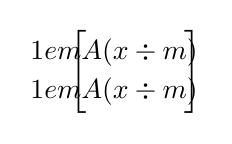
\begin{tikzpicture}[inner sep=1pt]
      \node (n1) at (0,-.25) {$\vecmatvec{1em}{A}{}{(x\div m)}$};
      \node (n2) at (0,.25) {$\vecmatvec{1em}{A}{}{(x\div m)}$};
      \node at (-.45, 0) {$\Bigg[$};
      \node at (1, 0) {$\Bigg]$};
   \end{tikzpicture}}}
 \\&&& =
   \vecmatvec{.5em}{}{A,M_2,A}{}
\end{align*}

\subsubsection{Quadratic Forms}
\begin{align*}
   \E[x^T A x] &= \mathrm{Tr}(A \Sigma) + \mu^T A \mu
   \\
   [\vecmatvec{.5em}{x}{A}{x}]
   &=
   [\vecmatvec{.5em}{(x\div \mu)}{A}{(x \div\mu)}
   +
   \vecmatvec{.5em}{\mu}{A}{\mu}]
   \\
   &=
   \mathbin{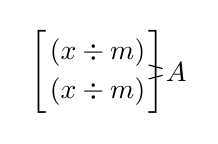
\begin{tikzpicture}[inner sep=1pt]
      \node (n1) at (0,-.25) {$(x\div m)$};
      \node (n2) at (0,.25) {$(x\div m)$};
      \node at (-.75, 0) {$\Bigg[$};
      \node at (.75, 0) {$\Bigg]$};
      \node (A) at (1, 0) {$A$};
      \draw (n1) -- (A);
      \draw (n2) -- (A);
   \end{tikzpicture}}
   +
   \vecmatvec{.5em}{\mu}{A}{\mu}
   \\
   &=
   \trace{\Sigma,A}2
   +
   \vecmatvec{.5em}{\mu}{A}{\mu}
\end{align*}

\subsubsection{Cubic Forms}

\subsection{Weighted Scalar Variable}
Let $y=w^T x$, and let $m=E[y]$, then
\begin{align*}
   \E[y] &= m = w^T \mu
   \\
   \E[(y-m)^2] &= \vecmatvec{.5em}{w}{M_2}{w}
   \\
   \E[(y-m)^3] &=
   \mathbin{\begin{tikzpicture}[baseline=(a0.base), inner sep=1pt]
      \node (a0) {$M_3$};
      \node[above=.3em of a0] (n0) {$w$};
      \node[right=.3em of a0] (n1) {$w$};
      \node[left=.3em of a0] (n3) {$w$};
      \draw (a0.north) -- (n0);
      \draw (a0.east) -- (n1);
      \draw (a0.west) -- (n3);
   \end{tikzpicture}}
   \\
   \E[(y-m)^4] &=
   \mathbin{\begin{tikzpicture}[baseline=(a0.base), inner sep=1pt]
      \node (a0) {$M_4$};
      \node[above=.3em of a0] (n0) {$w$};
      \node[right=.3em of a0] (n1) {$w$};
      \node[below=.3em of a0] (n2) {$w$};
      \node[left=.3em of a0] (n3) {$w$};
      \draw (a0.north) -- (n0);
      \draw (a0.east) -- (n1);
      \draw (a0.south) -- (n2);
      \draw (a0.west) -- (n3);
   \end{tikzpicture}}
\end{align*}
For specific distributions, like $x$ Gaussian, we can often reduce the moment tensors further.
Khintchine's inequality also gives a way to bound all of these in terms of $E[(y-m)^2]$.


\subsection{Gaussian Moments}
\subsubsection{Mean and covariance of linear forms}
\subsubsection{Mean and variance of square forms}
\subsubsection{Cubic forms}
\subsubsection{Mean of Quartic Forms}
\subsubsection{Gaussian Integration by Parts}
General principle for Gaussian expectations.


